\documentclass[main]{subfiles}

\begin{document}
    \subsection{(17.09.19) Поверхности}

    \begin{Example}
      \[\gamma: \R \ra \R^3, \q t \mapsto (r(t),\ 0,\ z(t)),\text{ где $r: \R \ra \R$, $z: \R \ra \R$}\]
      Найти параметрищацию поверхности вращения вокруг $OZ$
    \end{Example}

    \begin{proof}
      Из геометрических соображений: $(r(t) \cos \varphi,\ r(t)\sin \varphi,\ z(t)),\ \varphi \in [0,\ 2\pi]$\\
      Более строго:
      \[\begin{pmatrix}
        \cos \alpha & -\sin \alpha & 0\\
        \sin \alpha & \cos \alpha & 0\\
        0 & 0 & 1
      \end{pmatrix}
      \begin{pmatrix}
        r(t)\\
        0\\
        z(t)
      \end{pmatrix}
      =
      \begin{pmatrix}
        r(t) \cos \alpha\\
        r(t) \sin \alpha\\
        z(t)
      \end{pmatrix}\]
    \end{proof}

    \begin{definition}
      Гладкая двухмерная поверхность:
      \[F: \os{\text{откр}}{\us{t,\ s}{U}} \subset \R^2 \ra \R^3\]
      т.ч. $\dfrac{\d F}{\d S}$, $\dfrac{\d F}{\d t}$ - непрерывные функции
    \end{definition}

    \begin{definition}
      Гладкая регулярная поверхность:
      \[F: \os{\text{откр}}{\us{t,\ s}{U}} \subset \R^2 \ra \R^3\]
      т.ч. $\dfrac{\d F}{\d s}$, $\dfrac{\d F}{\d t}$ - линейно независимы\\
      "регулярная = скорость не обнуляется"
    \end{definition}
    \begin{figure}[H]
        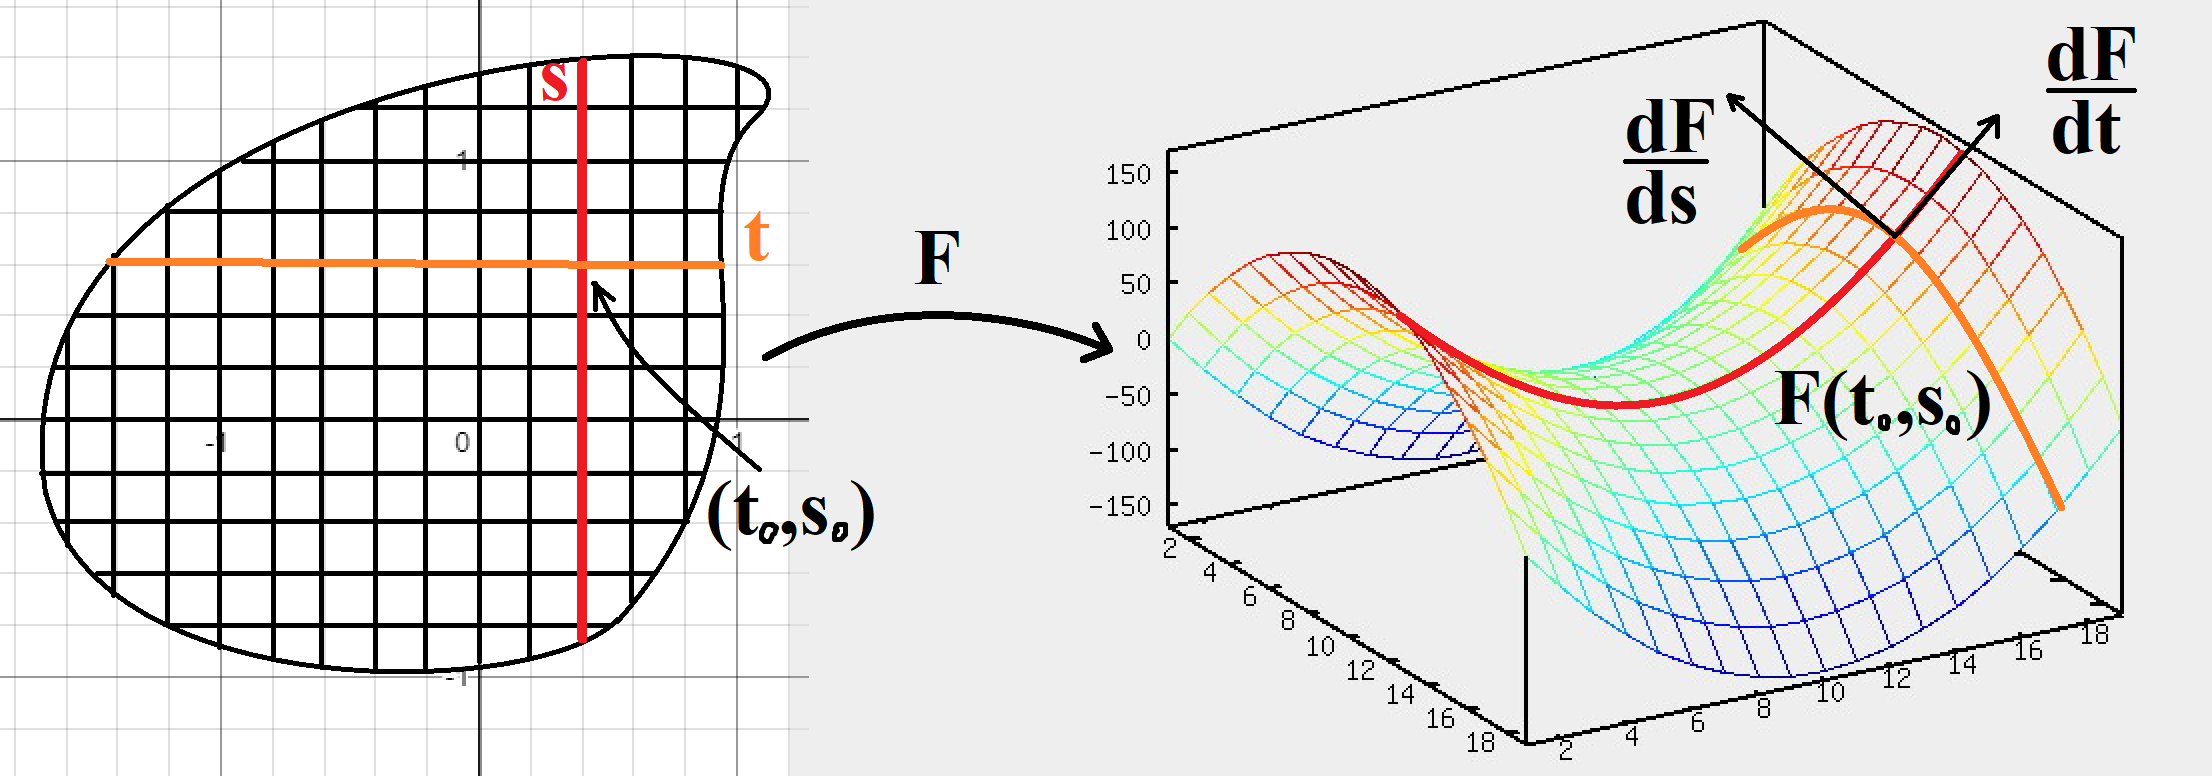
\includegraphics[scale=0.2]{pics/3_1.png}
        \centering
    \end{figure}
\end{document}
